\documentclass[12pt]{article}
\usepackage{amsmath}
\usepackage{amssymb}
\usepackage{geometry}
\usepackage{enumerate}
\usepackage{natbib}
\usepackage{float}%稳定图片位置
\usepackage{graphicx}%画图
\usepackage[english]{babel}
\usepackage{a4wide}
\usepackage{indentfirst}%缩进
\usepackage{enumerate}%加序号
\usepackage{multirow}%合并行


\begin{document}
\newpage
\section{(a)}
$$I_c=\frac{1}{2}\mu_nC_{ox}(\frac{W}{L})_3(V_c-V_{TH})^2=0.5*0.035*\frac{3.9*8.85*10^{-12}}{9*10^{-9}}*\frac{100}{2-2*0.08}*(1.2-0.7)^2=9.12\times10^{-4}(A)$$
$$A_{DM}=-\sqrt{\mu_nC_{ox}\frac{W}{L}I_c}R_D=-\sqrt{0.035*\frac{3.9*8.85*10^{-12}}{9*10^{-9}}*\frac{50}{2-2*0.08}*9.12\times10^{-4}}*5000=-9.12$$
$$A_{CM}=0$$
\section{(b)}
\begin{figure}[H]
\centering
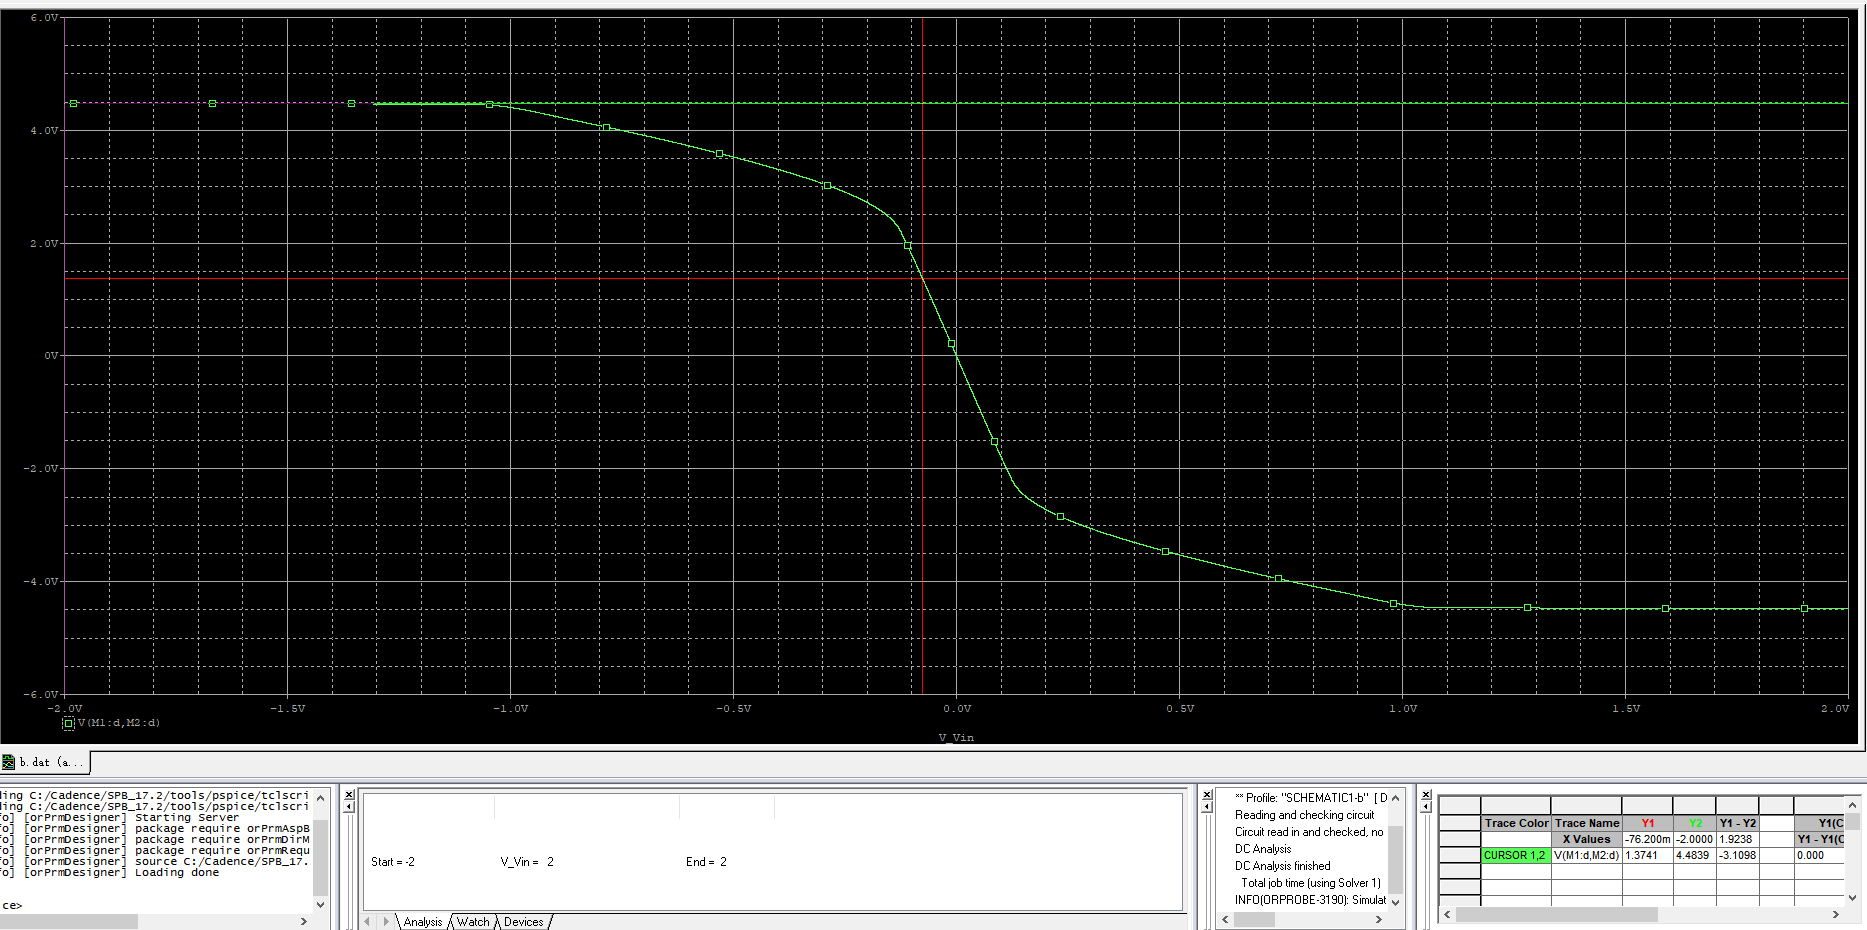
\includegraphics[scale=0.27]{P1.png}
\end{figure}
From the figure:
$$A_{DM}=\frac{1.3741}{-0.0762*2}=-9.016$$
The $A_{DM}$ from the figure is consistent to the calculated value.
\section{(c)}
\begin{figure}[H]
\centering
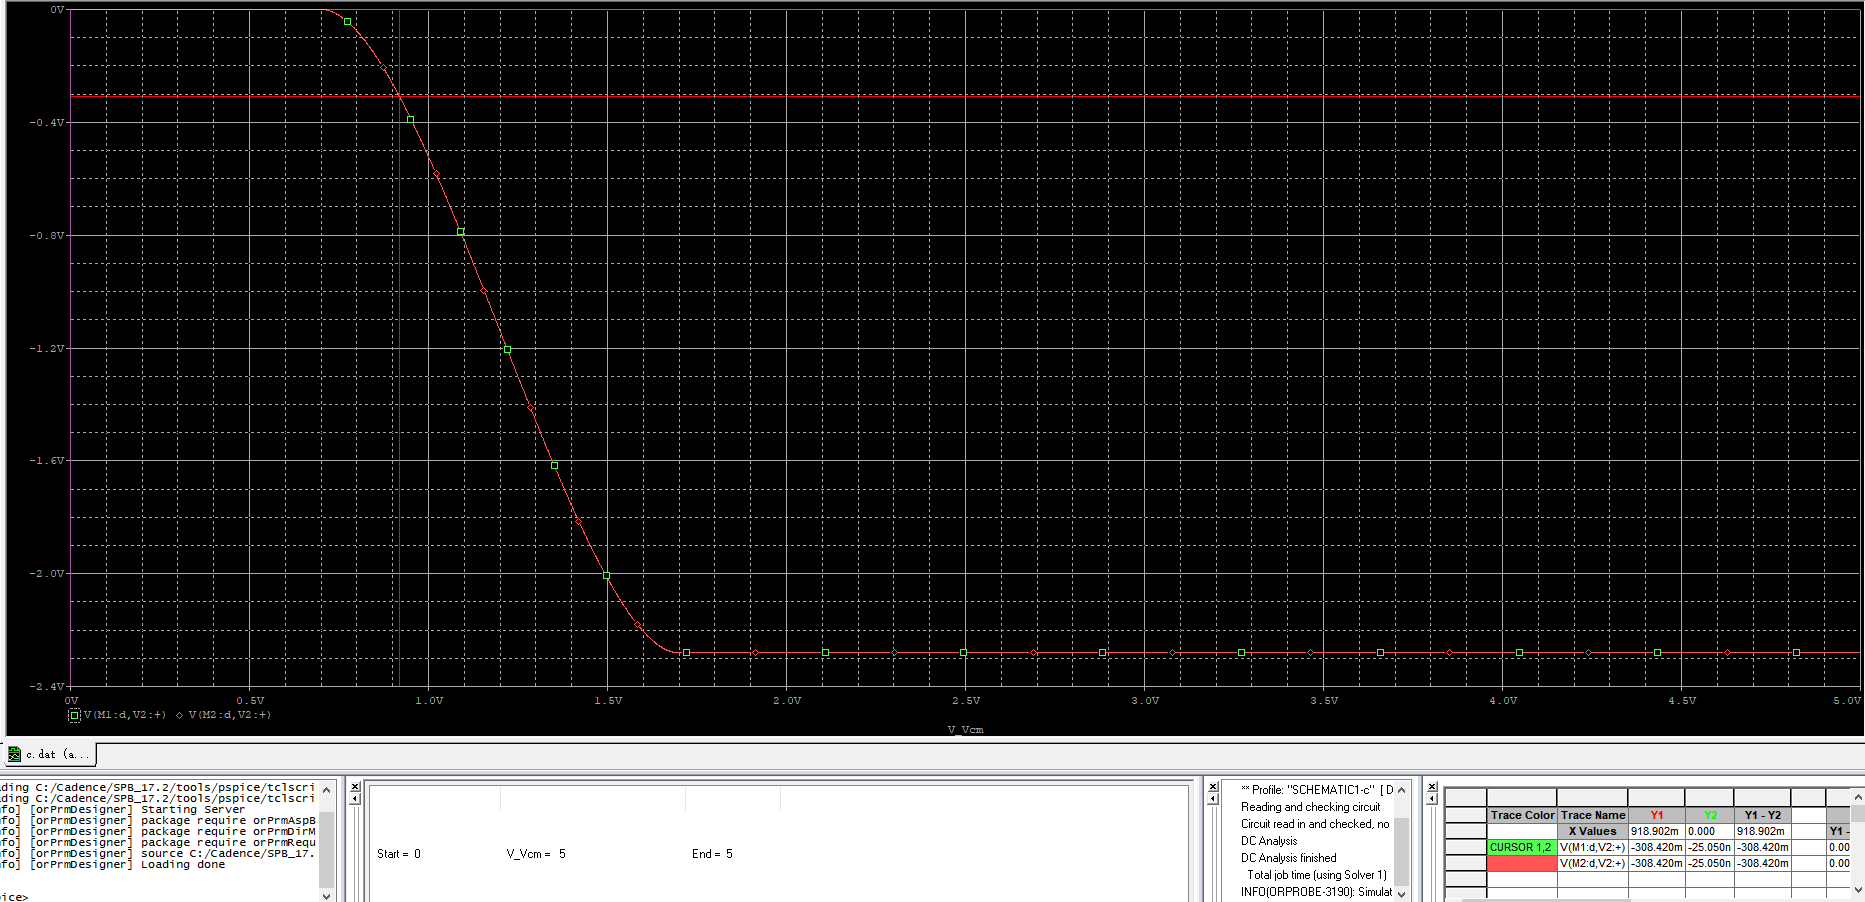
\includegraphics[scale=0.27]{P2.png}
\end{figure}
When $V_{CM}$ is large enough, $V_{out}$ no longer changes, which means $A_{CM}$ is close to $\infty$, and it's consistent to my calculated value.
\end{document}